\documentclass[11pt,a4paper]{article}
\usepackage[utf8]{inputenc}
\usepackage[expansion=false]{microtype}
\usepackage[a4paper,left=28mm,right=28mm,top=28mm,bottom=25mm]{geometry}
\usepackage{amsmath,amssymb}
\usepackage{booktabs}\usepackage{array}\usepackage{enumitem}\usepackage{xcolor}
\usepackage{caption}\usepackage{fancyhdr}\usepackage{titlesec}\usepackage{tikz}
\usetikzlibrary{positioning,arrows.meta,calc,fit,backgrounds,shapes.geometric}
\usepackage[most]{tcolorbox}\usepackage[section]{placeins}\usepackage[hidelinks]{hyperref}

\definecolor{navy}{RGB}{26,60,102}
\definecolor{accent}{RGB}{40,92,148}
\definecolor{softblue}{RGB}{232,240,248}
\definecolor{rulegrey}{RGB}{120,130,140}
\definecolor{orangeacc}{RGB}{196,106,48}
\definecolor{boxblue}{RGB}{219,232,244}
\definecolor{tealbox}{RGB}{214,236,238}
\definecolor{greybox}{RGB}{238,240,242}
\definecolor{greenbox}{RGB}{214,238,214}
\definecolor{goldbox}{RGB}{250,236,200}
\definecolor{pinkbox}{RGB}{250,216,224}

\hypersetup{colorlinks=true,linkcolor=accent,urlcolor=accent,citecolor=accent,
  pdftitle={Bluetooth Channel Sounding Inline Phase Transfer},
  pdfsubject={Formal technical report}}

\titleformat{\section}{\normalfont\Large\bfseries\color{navy}}{\thesection}{0.8em}{}
\titleformat{\subsection}{\normalfont\large\bfseries\color{navy}}{\thesubsection}{0.7em}{}
\titlespacing*{\section}{0pt}{1.9\baselineskip}{0.8\baselineskip}
\titlespacing*{\subsection}{0pt}{1.2\baselineskip}{0.5\baselineskip}
\captionsetup{font=small,labelfont={bf,color=accent},labelsep=colon,width=0.92\textwidth}
\captionsetup[table]{position=above,skip=4pt}
\captionsetup[figure]{position=below,skip=8pt}

\pagestyle{fancy}\fancyhf{}
\renewcommand{\headrulewidth}{0.6pt}
\fancyhead[L]{\small Bluetooth CS Inline Phase Transfer}
\fancyhead[R]{\small Formal technical report - Revision 1.0}
\fancyfoot[C]{\small\thepage}

\newtcolorbox{callout}[1][]{colback=softblue,colframe=accent,boxrule=0.5pt,
  left=6pt,right=6pt,top=5pt,bottom=5pt,arc=1pt,fontupper=\small,#1}
\newtcolorbox{caution}[1][]{colback=goldbox,colframe=orangeacc,boxrule=0.5pt,
  left=6pt,right=6pt,top=5pt,bottom=5pt,arc=1pt,fontupper=\small,#1}

\newcolumntype{L}[1]{>{\raggedright\arraybackslash}p{#1}}
\renewcommand{\arraystretch}{1.18}

\newcommand{\us}{\,\ensuremath{\upmu}s}
\newcommand{\PCT}{\ensuremath{\mathrm{PCT}}}
\newcommand{\IPT}{\ensuremath{\mathrm{IPT}}}
\newcommand{\FFO}{\ensuremath{\mathrm{FFO}}}
\newcommand{\FAE}{\ensuremath{\mathrm{FAE}}}
\newcommand{\RPL}{\ensuremath{\mathrm{RPL}}}
\newcommand{\TQI}{\ensuremath{\mathrm{TQI}}}
\newcommand{\NADM}{\ensuremath{\mathrm{NADM}}}
\newcommand{\Tsy}{T_{SY}}
\newcommand{\Tgd}{T_{GD}}
\newcommand{\Tsw}{T_{SW}}
\newcommand{\Tswipt}{T_{SW\_IPT}}
\newcommand{\Tpm}{T_{PM}}
\newcommand{\Trd}{T_{RD}}
\newcommand{\Tiptwo}{T_{IP2}}
\newcommand{\Nap}{N_{AP}}
\newcommand{\code}[1]{\texttt{\small #1}}
\providecommand{\upmu}{\mu}
\newcommand{\core}[1]{\textcolor{rulegrey}{\small[Core 6.3, #1]}}
\newcommand{\RTT}{\ensuremath{\mathrm{RTT}}}

\tikzset{
  blk/.style ={draw=navy!70,fill=softblue,rounded corners=1pt,align=center,font=\scriptsize,inner sep=3.5pt,minimum height=8mm},
  pblk/.style={draw=navy!70,fill=white,rounded corners=1pt,align=center,font=\scriptsize,inner sep=3.5pt,minimum height=8mm},
  ar/.style  ={-{Latex[length=2mm]},draw=navy!80,thick},
  dar/.style ={-{Latex[length=2mm]},draw=orangeacc,dashed,thin},
  slot/.style={draw=navy!55,font=\scriptsize,align=center,minimum height=7mm},
}

\begin{document}
\thispagestyle{empty}
\vspace*{18mm}
{\color{accent}\small\bfseries FORMAL TECHNICAL REPORT \hfill REVISION 1.0}
\vspace{26mm}

{\raggedright\color{navy}\Huge\bfseries Bluetooth Channel Sounding\par}
\vspace{5mm}
{\raggedright\color{navy}\huge\bfseries Inline Phase Transfer\par}

\vspace{7mm}
\noindent{\raggedright\color{rulegrey}\large Returning the reflector's phase in the radio signal
instead of the data path: the mechanism, the transmitter it demands, what it costs, what it removes,
and when to enable it\par}

\vspace{12mm}
\noindent\rule{\textwidth}{1pt}
\vspace{4mm}

\noindent
Inline PCT Transfer --- \IPT, and the subject of this report --- is an optional Channel Sounding
capability in which the reflector pre-rotates its outgoing tone by the phase it has just measured,
so that the initiator's own single-sided measurement already carries the full two-way channel phase.
The reflector's phase then no longer has to be transported anywhere: it has been returned
\emph{inline}, in the radio signal itself, and the phase correction term the reflector reports is
left with zero imaginary part, conveying amplitude alone. This report derives that mechanism from
the specification's own phase algebra, shows why the construction is exactly phase-neutral, and then
examines what it actually demands of a reflector: a transmitter whose carrier phase can be commanded
per antenna path, to a resolution that this report quantifies, and settled inside a switch period,
with the whole measure--compute--apply loop closed in as little as fifteen microseconds. It shows
that \IPT{} is thermally free --- the two-way phase variance is unchanged --- and that its real cost
is a new hardware term and the permanent loss of the reflector's phase as an auditable quantity. It
closes with the negotiation and configuration path, an error budget, a decision rule, and a
verification plan.

\vfill
\noindent
\begin{tabular}{@{}L{40mm}L{95mm}@{}}
Primary references & Core 6.3, Vol.\ 6, Part A, Sec.\ 6.5; Vol.\ 1, Part A, Sec.\ 9.2 \\
Step behaviour & Core 6.3, Vol.\ 6, Part H, Secs.\ 4.3.3, 4.3.4 and 4.6 \\
Capability and configuration & Core 6.3, Vol.\ 4, Part E; Vol.\ 6, Part B \\
Companion reports & \emph{Mode-0 Frequency and Timing Calibration}, Rev.\ 1.0;
                    \emph{Mode-1 RTT Estimation}, Rev.\ 1.0;
                    \emph{Mode-2 Phase-Based Ranging}, Rev.\ 1.0;
                    \emph{Mode-3 Combined RTT and PBR}, Rev.\ 1.0 \\
Document type & Scientific and implementation-oriented technical report \\
Revision date & 6 September 2026 \\
\end{tabular}

\newpage
\pagenumbering{roman}
\section*{Abstract}
\addcontentsline{toc}{section}{Abstract}

In ordinary phase-based ranging the two devices each measure the phase of the other's tone, each
reports a phase correction term, and a ranging entity multiplies the two complex terms together. The
product cancels the unknown relative local-oscillator phase and leaves twice the channel phase. That
construction requires both measurements to reach the same place, which means the reflector's phase
must travel back over some data path before any distance exists.

Inline PCT Transfer removes that requirement. With \IPT{} enabled, the reflector applies the phase it
has just measured to its own outgoing carrier \core{Vol.\ 6, Part A, Sec.\ 6.5}. The relative phase
the initiator then measures at its antenna is
$\theta_{INIT}(f) = \theta_{CH}(f) - \Delta\theta_{LO}(f) + \theta_{REFL}(f) = 2\theta_{CH}(f)$
\core{Vol.\ 1, Part A, Sec.\ 9.2}: the local-oscillator term cancels in the air rather than in
arithmetic, and the initiator holds the complete two-way observable from its own measurement alone.
The reflector's reported term becomes $\PCT_{REFL}(f) = A_{REFL}(f)e^{i0}$ --- the specification
requires the imaginary part to be zero and the real part to carry the measured amplitude --- so the
channel transfer function assembled by the ranging entity is unchanged.

This report treats \IPT{} as an engineering trade rather than a feature. Three findings frame it.
It is \emph{thermally free}: the two-way phase error is the sum of the same two independent phase
estimates as before, so the variance is identical and no precision is bought or lost. Its real cost
is a \emph{new hardware term}: the reflector must command its carrier phase per antenna path, and
this report shows that eight bits of applied-phase resolution costs $2.5\%$ of ranging precision
while six bits costs $34\%$. And it is \emph{irreversible}: because the correction is applied in the
radio rather than recorded, the reflector's phase estimate can never be re-examined, re-processed or
audited, and the diagnostic separation between initiator-side and reflector-side error is gone for
good. The report quantifies the real-time budget the reflector must close --- as little as $15\us$
between measuring a path and transmitting it --- explains the separate $\Tswipt$ and
$\Tiptwo$ capability declarations that exist because of it, and argues that \IPT{} pairs naturally
with Mode-3, whose round-trip time restores the independent check that \IPT{} removes.

\begin{callout}
\textbf{Status and interpretation.} Normative claims are tied to the cited Bluetooth Core
Specification sections and have been checked against the adopted Core 6.3 text. The error analysis,
the applied-phase resolution study, the real-time budget, the decision rule and the verification plan
are this report's own and are not specified. The Bluetooth specification and adopted test
specifications remain authoritative for conformance.
\end{callout}

\newpage
\tableofcontents
\newpage
\pagenumbering{arabic}
\setcounter{page}{1}

% ============================================================
\section{Scope, naming, and what \IPT{} changes}
% ============================================================

\subsection{Naming}

The specification uses two names for one capability. Volume 1, Part A calls it \emph{Channel Sounding
Inline Phase Correction Term Transfer}; Volume 6, Part A, Section 6.5 calls it \emph{Inline PCT
Transfer} and abbreviates it \IPT, which is the form used in the link-layer and host-interface
parameter names. It is colloquially called \emph{inline phase-based ranging} or \emph{inline PBR},
because its effect is to complete a phase-based ranging measurement inside the radio exchange. This
report uses \IPT{} throughout.

\IPT{} is a \emph{reflector} capability. It is declared by the reflector, enabled by configuration,
and it changes what the reflector transmits and what it reports; the initiator's own measurement and
reporting format are untouched \core{Vol.\ 4, Part E}.

\subsection{The problem it solves}

The companion Mode-2 report develops the ordinary construction. Each device measures the phase of the
other's tone against its own oscillator; each reports a phase correction term; the ranging entity
multiplies the two complex terms, and the unknown relative oscillator phase cancels in the product.
The construction is exact and needs no shared time base --- but it needs both halves in one place.

That requirement is the whole motivation for \IPT. Until the reflector's phase correction terms reach
whatever computes the range, no distance exists. In a system where the initiator is the device that
needs the answer, those terms must traverse the reflector's controller, its host, and the connection
back to the initiator, for every tone on every channel. The measurement is finished in microseconds;
the answer waits on a data path.

\begin{callout}
\textbf{What \IPT{} moves.} It does not make the measurement better and it does not make it faster in
the radio. It moves \emph{where the two-way phase is formed} --- out of the ranging entity's
arithmetic and into the reflector's transmitter. The consequence is that the initiator's own
measurement is already the answer, so the ranging-critical half of the data no longer has to be
carried anywhere.
\end{callout}

\subsection{What this report covers}

Sections~\ref{sec:mech} and~\ref{sec:reflector} derive the mechanism and the transmitter it demands.
Section~\ref{sec:timing} covers the timing parameters that exist only because of \IPT.
Section~\ref{sec:report} covers the altered reporting.
Section~\ref{sec:negotiation} covers capability and configuration.
Sections~\ref{sec:error}--\ref{sec:lost} are the engineering assessment: what changes in the error
budget, and what is permanently given up.
Sections~\ref{sec:integrity}--\ref{sec:decision} cover integrity and the decision to enable it.
The remainder follows the pattern of the companion reports.
% ============================================================
\section{Normative framework and terminology}
% ============================================================

\begin{table}[h]
\caption{Normative map for Inline PCT Transfer.}
\label{tab:normmap}
\centering\small
\begin{tabular}{@{}L{42mm}L{51mm}L{51mm}@{}}
\toprule
Source & What it defines & Question answered \\
\midrule
Core 6.3, Vol.\ 1, Part A, Sec.\ 9.2 & The phase algebra, with and without \IPT & Why does the initiator's own measurement suffice? \\
Core 6.3, Vol.\ 6, Part A, Sec.\ 6.5 & \IPT\ normative behaviour: $Q=0$, phase accuracy, carrier adjustment & What must the reflector do? \\
Core 6.3, Vol.\ 6, Part A, Sec.\ 6.2 & Phase measurement accuracy requirements, which still apply & To what accuracy? \\
Core 6.3, Vol.\ 6, Part H, Sec.\ 4.3.3 & Mode-2 step; $\Tswipt$; tone extension slot exemption under \IPT & How does the step change? \\
Core 6.3, Vol.\ 6, Part H, Sec.\ 4.3.4 & Mode-3 step, to which \IPT\ equally applies & Does \IPT\ work with Mode-3? \\
Core 6.3, Vol.\ 6, Part H, Sec.\ 4.6 & $\PCT$ encoding, reference power level, tone quality & How is the result reported? \\
Core 6.3, Vol.\ 6, Part B & \code{LL\_CS\_CAPABILITIES} exchange and configuration defaults & How is \IPT\ negotiated? \\
Core 6.3, Vol.\ 4, Part E & \code{Subfeatures\_Supported} bit 4, \code{CS\_Enhancements} bit 0, $\Tiptwo$/$\Tswipt$ time lists & How is it declared and enabled? \\
\bottomrule
\end{tabular}
\end{table}

\begin{table}[h]
\caption{Principal symbols. The phase symbols follow Volume 1, Part A, Section 9.2.}
\label{tab:symbols}
\centering\small
\begin{tabular}{@{}L{34mm}L{72mm}L{22mm}@{}}
\toprule
Symbol & Meaning & Units \\
\midrule
$\theta_{CH}(f)$ & One-way phase delay of the channel & rad \\
$\Delta\theta_{LO}(f)$ & Relative phase difference of the two devices' carriers & rad \\
$\theta_{REFL}(f)$ & Phase measured at the reflector's antenna & rad \\
$\theta_{INIT}(f)$ & Phase measured at the initiator's antenna & rad \\
$A_{REFL},A_{INIT}$ & Measured carrier amplitudes at each device & --- \\
$\PCT_{REFL},\PCT_{INIT}$ & Reported phase correction terms, complex & --- \\
$H_2(f)$ & Assembled two-way channel transfer function & --- \\
$\varphi_{app}$ & Phase the reflector applies to its outgoing carrier & rad \\
$b$ & Applied-phase resolution of the reflector's transmitter & bits \\
$\Tswipt$ & Antenna switch period declared for \IPT\ operation & s \\
$\Tiptwo$ & Interlude period, from the \IPT\ time list when \IPT\ is enabled & s \\
$\RPL$ & Reference power level accompanying the $\PCT$ values & dBm \\
$\sigma_\theta$ & Per-tone phase estimation standard deviation & rad \\
$\sigma_\Theta$ & Two-way phase standard deviation & rad \\
\bottomrule
\end{tabular}
\end{table}

% ============================================================
\section{The mechanism}
\label{sec:mech}
% ============================================================

\subsection{The ordinary construction}

Volume 1, Part A, Section 9.2 sets out the baseline. With $\theta_{CH}(f)$ the one-way channel phase
and $\Delta\theta_{LO}(f)$ the relative carrier phase between the devices, the phases measured at the
two antennas are
\begin{equation}
\theta_{REFL}(f) = \theta_{CH}(f) + \Delta\theta_{LO}(f),
\qquad
\theta_{INIT}(f) = \theta_{CH}(f) - \Delta\theta_{LO}(f),
\label{eq:baseline}
\end{equation}
and each device reports a phase correction term carrying that phase together with the measured
amplitude,
\begin{equation}
\PCT_{REFL}(f) = A_{REFL}(f)\,e^{i\theta_{REFL}(f)},
\qquad
\PCT_{INIT}(f) = A_{INIT}(f)\,e^{i\theta_{INIT}(f)} .
\label{eq:pcts}
\end{equation}
The ranging entity forms the product, and the oscillator term cancels:
\begin{equation}
H_2(f) \;=\; \PCT_{REFL}(f)\,\PCT_{INIT}(f) \;=\; A_{CH2}(f)\,e^{i2\theta_{CH}(f)} .
\label{eq:H2}
\end{equation}
Note where the cancellation happens: in a multiplication, performed wherever both terms have arrived.

\subsection{The inline construction}

With \IPT{} enabled the reflector does not merely measure $\theta_{REFL}$; it applies that phase to
its own outgoing carrier \core{Vol.\ 6, Part A, Sec.\ 6.5}. The phase the initiator subsequently
measures at its antenna therefore carries the reflector's measurement as well as the channel:
\begin{equation}
\theta_{INIT}(f)
 \;=\; \theta_{CH}(f) - \Delta\theta_{LO}(f) + \theta_{REFL}(f)
 \;=\; \theta_{CH} - \Delta\theta_{LO} + \theta_{CH} + \Delta\theta_{LO}
 \;=\; 2\theta_{CH}(f) ,
\label{eq:inline}
\end{equation}
which is the relation given in Volume 1, Part A, Section 9.2. The unknown relative oscillator phase
has cancelled --- but it has cancelled \emph{in the air}, between the reflector's transmitter and the
initiator's receiver, rather than in an arithmetic product formed later.

Because the reflector has already handed over its phase, the term it reports carries none:
\begin{equation}
\PCT_{REFL}(f) \;=\; A_{REFL}(f)\,e^{i0} ,
\label{eq:pctrefl}
\end{equation}
and the assembled transfer function is unchanged from Eq.~\eqref{eq:H2},
\begin{equation}
H_2(f) \;=\; A_{REFL}(f)e^{i0} \times A_{INIT}(f)e^{i\theta_{INIT}(f)}
 \;=\; A_{CH2}(f)\,e^{i2\theta_{CH}(f)} .
\label{eq:H2ipt}
\end{equation}

\begin{figure}[h]
\centering
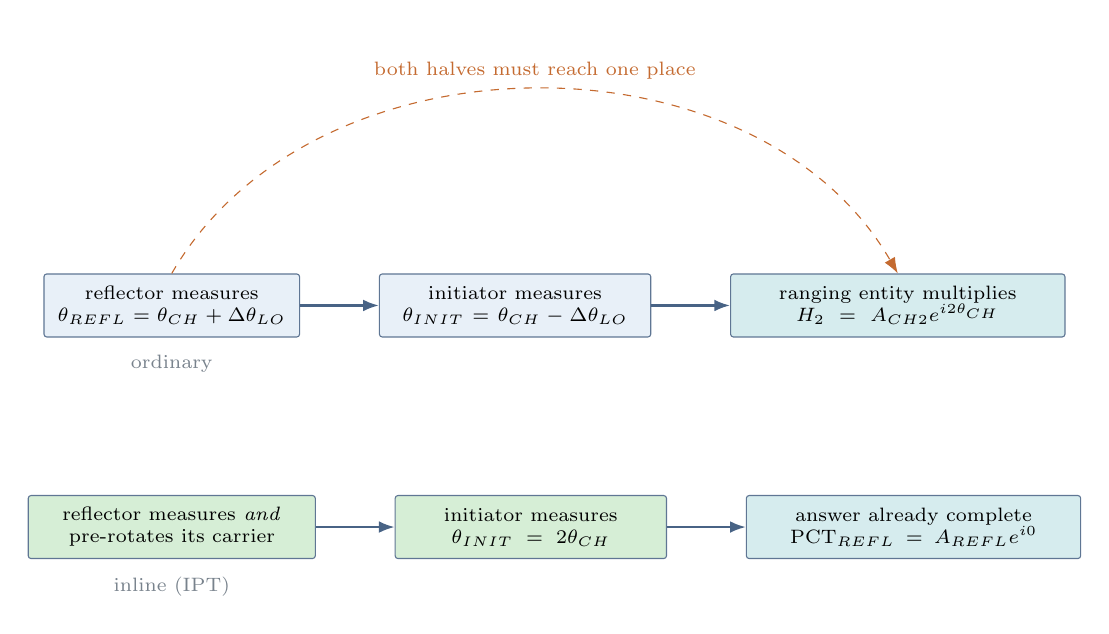
\begin{tikzpicture}[node distance=6mm and 8mm]
\node[blk,text width=30mm] (r1) {reflector measures\\ $\theta_{REFL}=\theta_{CH}+\Delta\theta_{LO}$};
\node[blk,right=10mm of r1,text width=32mm] (i1) {initiator measures\\ $\theta_{INIT}=\theta_{CH}-\Delta\theta_{LO}$};
\node[blk,right=10mm of i1,text width=40mm,fill=tealbox] (p1) {ranging entity multiplies\\ $H_2=A_{CH2}e^{i2\theta_{CH}}$};
\draw[ar] (r1)--(i1); \draw[ar] (i1)--(p1);
\node[font=\scriptsize,color=rulegrey,anchor=north] at ($(r1.south)+(0,-1mm)$) {ordinary};
\draw[dar] (r1.north) to[out=60,in=120] node[midway,above,font=\scriptsize,color=orangeacc]
   {both halves must reach one place} (p1.north);

\node[blk,below=20mm of r1,text width=34mm,fill=greenbox] (r2) {reflector measures \emph{and}\\ pre-rotates its carrier};
\node[blk,right=10mm of r2,text width=32mm,fill=greenbox] (i2) {initiator measures\\ $\theta_{INIT}=2\theta_{CH}$};
\node[blk,right=10mm of i2,text width=40mm,fill=tealbox] (p2) {answer already complete\\ $\PCT_{REFL}=A_{REFL}e^{i0}$};
\draw[ar] (r2)--(i2); \draw[ar] (i2)--(p2);
\node[font=\scriptsize,color=rulegrey,anchor=north] at ($(r2.south)+(0,-1mm)$) {inline (\IPT)};
\end{tikzpicture}
\caption{Where the two-way phase is formed. Ordinarily the cancellation of $\Delta\theta_{LO}$
happens in a product computed once both phase correction terms have arrived somewhere. With \IPT{}
it happens in the radio link itself, and the initiator's single measurement is already
$2\theta_{CH}$.}
\label{fig:mech}
\end{figure}

\begin{callout}
\textbf{The identity that makes it work.} Equation~\eqref{eq:inline} is exact and requires no
assumption beyond the channel reciprocity already assumed in Eq.~\eqref{eq:baseline}. The reflector's
measurement carries $+\Delta\theta_{LO}$ and the initiator's carries $-\Delta\theta_{LO}$; adding one
to the other in the radio is algebraically the same operation as multiplying the two complex terms
later. \IPT{} is therefore not an approximation of ordinary phase-based ranging --- it is the same
computation, relocated.
\end{callout}

\subsection{What the initiator must still be given}

Equation~\eqref{eq:H2ipt} still contains $A_{REFL}(f)$, and the reflector still reports it in the
real part of its phase correction term. For a range extracted from the \emph{slope} of
$\arg H_2$ against frequency, the reflector's amplitude is irrelevant: it affects only the magnitude.
For a range extracted from the \emph{inverse transform} --- the channel impulse response of the
companion Mode-2 report --- the amplitude is a weighting, and discarding it changes the shape of the
point-spread function and hence first-path detection.

\begin{callout}
\textbf{A useful robustness property, and its limit.} With \IPT{} the initiator can compute a
phase-slope range from its own measurements alone, so a lost or delayed reflector report degrades the
result rather than preventing it. That is a real availability gain. It does not extend to
transform-domain processing, which wants $A_{REFL}$ as a weight --- so an implementation that relies
on first-path detection has not escaped the reverse data path, only made it non-blocking.
\end{callout}
% ============================================================
\section{What \IPT{} demands of the reflector}
\label{sec:reflector}
% ============================================================

Equation~\eqref{eq:inline} is one line of algebra. Implementing it is a transmitter requirement, and
it is the substance of the feature.

\subsection{A phase-commandable transmitter}

The reflector must be able to set the phase of its transmitted carrier to a commanded value, per
antenna path, per channel. Nothing in ordinary Channel Sounding requires this: a conventional
reflector transmits an unmodulated tone whose absolute phase is arbitrary, because the ordinary
construction never depends on it. Under \IPT{} that arbitrary phase becomes the observable, and it
must be placed deliberately.

Three implementation routes are common, and they differ in exactly the properties that
Section~\ref{sec:error} shows to matter.

\begin{table}[h]
\caption{Routes to a phase-commandable carrier, and the properties that bear on ranging.}
\label{tab:routes}
\centering\small
\begin{tabular}{@{}L{34mm}L{34mm}L{30mm}L{28mm}@{}}
\toprule
Mechanism & Resolution & Settling & Principal risk \\
\midrule
Direct digital synthesis of the tone at baseband, upconverted & Set by the numerically controlled oscillator word; easily 12 bits or more & Immediate, in the digital domain & Image and DC leakage rotate the effective phase \\
Programmable phase shifter in the RF path & Set by the shifter, often 5--8 bits & Device-dependent; must fit inside $\Tswipt$ & Amplitude--phase coupling; state-dependent insertion loss \\
Phase-continuous synthesiser retune & Fine, but indirect & Slowest; may not fit a $1\us$ switch period & Settling transient inside $\Tpm$ \\
\bottomrule
\end{tabular}
\end{table}

\begin{callout}
\textbf{Applied-phase resolution is a ranging specification.} Section~\ref{sec:error} quantifies it:
at the worked configuration, eight bits of applied-phase resolution costs $2.5\%$ of ranging
precision and six bits costs $34\%$. A five- or six-bit RF phase shifter, entirely adequate for
beam-steering, is not adequate here. This is the single most likely way for an \IPT{} implementation
to be quietly worse than the non-\IPT{} implementation it replaced.
\end{callout}

\subsection{The real-time loop}

The reflector must measure a path's phase, compute the value to apply, program the transmitter, and
have the carrier settled before its own tone slot for that path opens. The available margin follows
from the Mode-2 step structure of the companion report: the reflector's tone sequence begins after
the initiator's sequence, its ramp-down and the interlude, and the reflector transmits its antenna
paths in the same order it measured them, so the margin is very nearly the same for every path:
\begin{equation}
T_{margin} \;\approx\; \Trd \;+\; \Tiptwo .
\label{eq:margin}
\end{equation}

\begin{table}[h]
\caption{Real-time margin available to the reflector's measure--compute--apply loop, from
Eq.~\eqref{eq:margin} with $\Trd = 5\us$.}
\label{tab:margin}
\centering\small
\begin{tabular}{@{}rrL{74mm}@{}}
\toprule
$\Tiptwo$ & $T_{margin}$ & Comment \\
\midrule
$10\us$  & $15\us$  & The shortest configuration; demands a hardware-paced pipeline \\
$20\us$  & $25\us$  & Feasible for a tightly written firmware loop \\
$40\us$  & $45\us$  & Comfortable; the value used in the worked example \\
$80\us$  & $85\us$  & Generous \\
$145\us$ & $150\us$ & Mandatory value; ample, but lengthens the step and the reciprocal interval \\
\bottomrule
\end{tabular}
\end{table}

\begin{caution}
\textbf{The interlude is not free to lengthen.} Relaxing $\Tiptwo$ to buy computation time directly
lengthens $\Delta T$, the interval between the two reciprocal tone measurements, which the companion
Mode-2 report shows enters the range as $c\,\epsilon\,\Delta T/2$ against the residual frequency
offset. Moving from $\Tiptwo = 10\us$ to $145\us$ multiplies that term by roughly a factor of nine.
An \IPT{} implementation that needs a long interlude to close its loop is spending ranging accuracy
to buy processing time, and should account for it explicitly rather than treating the interlude as a
free parameter.
\end{caution}

\subsection{The phase accuracy requirement still applies}

Section 6.5 states plainly that ``a CS reflector shall satisfy the phase accuracy requirements''
\core{Vol.\ 6, Part A, Secs.\ 6.5 and 6.2}. Enabling \IPT{} does not relax the conformance limits on
the phase chain; it changes where in the chain the phase appears. The linear-regression bounds of
Section 6.2 --- a fitted slope below $2\pi\times1.7$\,ns and residuals below $0.28$\,rad for 95\% of
values --- must still be met, and under \IPT{} the reflector's applied-phase error is inside the loop
those bounds constrain.

\subsection{The tone extension slot is exempt}

One explicit relaxation exists. When \IPT{} is enabled, ``there is no requirement to compensate the
phase of the CS tone over the CS tone extension slot''
\core{Vol.\ 6, Part H, Sec.\ 4.3.3}. The extension slot exists as a noise and interference reference
and as a duration-matching device, not as a ranging observable, so there is no measured phase to
return for it. An implementation should not treat the extension slot's phase as meaningful under
\IPT, and a receiver should not include it in a slope fit.

% ============================================================
\section{Timing parameters that exist only for \IPT}
\label{sec:timing}
% ============================================================

Because the reflector's transmitter now has work to do between slots, the specification gives \IPT{}
its own declarations for the two periods that bound that work
\core{Vol.\ 4, Part E; Vol.\ 6, Part H, Sec.\ 4.3}.

\begin{table}[h]
\caption{The \IPT-specific timing declarations. Both are declared by the reflector alongside, and
independently of, the ordinary values.}
\label{tab:iptt}
\centering\small
\begin{tabular}{@{}L{34mm}L{44mm}L{54mm}@{}}
\toprule
Parameter & Declared values & Purpose \\
\midrule
$\Tswipt$ & 0, 1, 2, 4 or $10\us$ --- the same set as $\Tsw$, declared separately & The antenna switch period used when \IPT\ is enabled, within which the new phase must also settle \\
$\Tiptwo$ \IPT\ time list & Bits for 10, 20, 30, 40, 50, 60 and $80\us$; $145\us$ remains mandatory and is not in the optional list & The interlude the reflector can support while closing its measure--compute--apply loop \\
\bottomrule
\end{tabular}
\end{table}

Two observations follow from the value sets.

\emph{$\Tswipt$ buys no extra time by itself.} Its permitted values are identical to those of
$\Tsw$, so a reflector cannot ask for a longer switch period than the ordinary maximum of $10\us$.
What the separate declaration provides is the ability to declare a \emph{different} value --- a
reflector whose phase shifter settles in $4\us$ may support $\Tsw = 1\us$ without \IPT{} and require
$\Tswipt = 4\us$ with it, and the two are negotiated independently. In the step-duration formulas,
$\Tsw$ and $\Tswipt$ are represented by the same symbol \core{Vol.\ 6, Part H, Secs.\ 4.3.3
and 4.3.4}, so the arithmetic of the companion Mode-2 and Mode-3 reports is unchanged; only which
value is substituted differs.

\emph{The $\Tiptwo$ \IPT{} list is where the real accommodation is.} A reflector that cannot close
Eq.~\eqref{eq:margin} at $10\us$ simply does not set that bit, and the configuration must then choose
a longer interlude --- with the accuracy consequence noted above.

% ============================================================
\section{Altered reporting}
\label{sec:report}
% ============================================================

\subsection{The zero-quadrature rule}

Under \IPT{} the reflector ``shall only return PCT values where the imaginary (Q) part of each PCT
value is zero'', and ``the real (I) part of the PCT is used to convey the measured signal amplitude''
\core{Vol.\ 6, Part A, Sec.\ 6.5}. Volume 6, Part H adds that the real part ``shall be non-negative
and should reflect the magnitude of measurement'' \core{Vol.\ 6, Part H, Sec.\ 4.6}, and the host
interface repeats the rule at the event level, noting that ``on the initiator side, the Tone\_PCT
format remains unchanged'' \core{Vol.\ 4, Part E}.

\begin{table}[h]
\caption{What each device reports per tone, with and without \IPT.}
\label{tab:reporting}
\centering\small
\begin{tabular}{@{}L{30mm}L{45mm}L{45mm}@{}}
\toprule
 & Without \IPT & With \IPT \\
\midrule
Reflector $\PCT$ & 12-bit signed $I$ and $Q$; carries $A_{REFL}e^{i\theta_{REFL}}$ & $Q \equiv 0$; $I$ non-negative, carries $A_{REFL}$ only \\
Initiator $\PCT$ & 12-bit signed $I$ and $Q$; carries $A_{INIT}e^{i\theta_{INIT}}$ & Unchanged; now carries $A_{INIT}e^{i2\theta_{CH}}$ \\
Reference power level & 8-bit signed dBm, one per subevent & Unchanged \\
Tone quality indicator & 2-bit, per tone & Unchanged \\
Information in the reflector's report & Phase and amplitude & Amplitude only \\
\bottomrule
\end{tabular}
\end{table}

The field widths do not change: the reflector still emits a 24-bit \code{Tone\_PCT} per tone, half of
which is now known in advance to be zero. \IPT{} therefore saves nothing in the host interface's
event size. What it saves is the \emph{dependency}, not the bytes --- the ranging-critical phase no
longer has to arrive for a range to exist.

\subsection{Amplitude and the reference power level}

The reference power level is unaffected: it remains an 8-bit signed dBm value, one per subevent,
against which the unitless $I$ and $Q$ are interpreted through
\begin{equation}
\mathrm{IQ}_{\mathrm{dBm}} \;=\; 20\log_{10}\!\left(\frac{|\mathrm{IQ}_{linear}|}{2048}\right) + \RPL_{\mathrm{dBm}}
\label{eq:rpl}
\end{equation}
\core{Vol.\ 6, Part H, Sec.\ 4.6}. Under \IPT{} the reflector's $|\mathrm{IQ}|$ is simply its $I$
value, so Eq.~\eqref{eq:rpl} still yields a calibrated received power at the reflector --- which is
worth retaining, because it is the only remaining window into what the reflector actually saw.
% ============================================================
\section{Capability negotiation and configuration}
\label{sec:negotiation}
% ============================================================

\IPT{} is optional, is a property of the reflector role, and is off unless deliberately switched on.

\begin{enumerate}[leftmargin=1.6em,itemsep=2pt]
  \item \textbf{Prerequisite feature.} \IPT{} sits under the Channel Sounding Enhancement~\#1 LE
    feature; the \IPT-specific time lists are meaningful only if that feature is supported
    \core{Vol.\ 4, Part E}.
  \item \textbf{Capability declaration.} In its \code{Subfeatures\_Supported} field the reflector
    sets bit 4, ``IPT in the CS reflector'', and it populates the two \IPT{} time lists tabulated
    in Appendix~\ref{app:hci}. A device that does not support \IPT{} in the reflector role sets
    $\Tswipt$ to zero \core{Vol.\ 4, Part E}.
  \item \textbf{Link-layer exchange.} The declaration travels between the devices in the version-2
    \code{LL\_CS\_CAPABILITIES} request and response PDUs \core{Vol.\ 6, Part B}.
  \item \textbf{Configuration.} \IPT{} is enabled by bit 0, ``IPT is enabled in the CS reflector'',
    of the \code{CS\_Enhancements} configuration octet \core{Vol.\ 4, Part E}.
  \item \textbf{Default.} The specification is explicit that the parameter ``shall be set by default
    to not enabled and may be set to enabled if support for \IPT{} was indicated in the peer's
    \code{LL\_CS\_CAPABILITIES\_REQ} [v2] or \code{LL\_CS\_CAPABILITIES\_RSP} [v2] PDU''
    \core{Vol.\ 6, Part B}.
\end{enumerate}

\begin{callout}
\textbf{Both roles must know.} The reflector changes what it transmits; the initiator must know that
the reflector's reported quadrature is meaningless and that its own measurement is already the
two-way phase. An initiator that applies the ordinary product of Eq.~\eqref{eq:H2} to an \IPT{}
reflector's report multiplies by a purely real number and obtains $A_{CH2}e^{i2\theta_{CH}}$ ---
which happens to be correct. An initiator that instead \emph{adds} unwrapped angles, as the companion
Mode-2 report warns against, adds zero and also obtains the right answer. The dangerous case is the
reverse: an initiator that assumes \IPT{} when it is not enabled will treat
$\theta_{CH}-\Delta\theta_{LO}$ as $2\theta_{CH}$ and produce a confidently wrong range contaminated
by the oscillator phase. The configuration state must be read, not inferred from a zero quadrature.
\end{callout}

% ============================================================
\section{Error analysis}
\label{sec:error}
% ============================================================

\subsection{\IPT{} is thermally free}

It is worth establishing this carefully, because the intuition that returning a measurement through
the radio must cost something is wrong.

Without \IPT, the two-way phase is the sum of two independent estimates. Writing $\varepsilon_R$ and
$\varepsilon_I$ for the estimation errors at the reflector and initiator, each of variance
$\sigma_\theta^2$,
\begin{equation}
\arg H_2 \;=\; 2\theta_{CH} + \varepsilon_R + \varepsilon_I,
\qquad
\sigma_\Theta^2 \;=\; 2\sigma_\theta^2 .
\label{eq:noipt}
\end{equation}

With \IPT, the reflector applies its \emph{estimate} $\theta_{REFL}+\varepsilon_R$ to the carrier.
The initiator then measures that, with its own error:
\begin{equation}
\theta_{INIT} \;=\; \theta_{CH} - \Delta\theta_{LO} + \bigl(\theta_{REFL}+\varepsilon_R\bigr) + \varepsilon_I
 \;=\; 2\theta_{CH} + \varepsilon_R + \varepsilon_I ,
\label{eq:ipterr}
\end{equation}
which is term for term the same as Eq.~\eqref{eq:noipt}.

\begin{callout}
\textbf{The same two errors, combined the same way.} \IPT{} does not average, duplicate or amplify the
phase estimates; it relocates the addition. Both constructions accumulate exactly one reflector-side
and one initiator-side phase error, so the thermal precision of the companion Mode-2 report ---
$\sigma_\Theta = \sqrt2\,\sigma_\theta$, giving $4.065$\,mm over the full 72-channel raster at
20\,dB --- carries across to \IPT{} unchanged. Any claim that \IPT{} is inherently more or less
precise is mistaken; what differs is the hardware term below.
\end{callout}

\subsection{The term \IPT{} adds}

What \IPT{} does introduce is an error that does not exist otherwise: the reflector's applied phase
is not exactly the phase it intended. Write $\eta$ for that applied-phase error, so that
Eq.~\eqref{eq:ipterr} becomes $2\theta_{CH} + \varepsilon_R + \varepsilon_I + \eta$.

The dominant contribution to $\eta$ in most implementations is the resolution of whatever sets the
carrier phase. For a uniform quantiser of $b$ bits over $2\pi$,
\begin{equation}
\sigma_\eta \;=\; \frac{2\pi}{2^{b}\sqrt{12}} .
\label{eq:quant}
\end{equation}

\begin{table}[h]
\caption{Cost of applied-phase resolution, evaluated on the full 72-channel CS raster at
$\gamma = 20$\,dB and $\Tpm = 10\us$, where the baseline two-way phase noise is $1.812^{\circ}$ and
the baseline ranging precision is $4.065$\,mm.}
\label{tab:resolution}
\centering\small
\begin{tabular}{@{}rrrrr@{}}
\toprule
$b$ & Applied-phase LSB & $\sigma_\eta$ & Its own $\sigma_d$ & Combined $\sigma_d$ \\
\midrule
6  & $5.625^{\circ}$ & $1.624^{\circ}$ & $3.643$\,mm & $5.458$\,mm \ ($+34.3\%$) \\
7  & $2.812^{\circ}$ & $0.812^{\circ}$ & $1.821$\,mm & $4.454$\,mm \ ($+9.6\%$) \\
8  & $1.406^{\circ}$ & $0.406^{\circ}$ & $0.911$\,mm & $4.166$\,mm \ ($+2.5\%$) \\
9  & $0.703^{\circ}$ & $0.203^{\circ}$ & $0.455$\,mm & $4.090$\,mm \ ($+0.6\%$) \\
10 & $0.352^{\circ}$ & $0.101^{\circ}$ & $0.228$\,mm & $4.071$\,mm \ ($+0.2\%$) \\
12 & $0.088^{\circ}$ & $0.025^{\circ}$ & $0.057$\,mm & $4.065$\,mm \ ($+0.0\%$) \\
\bottomrule
\end{tabular}
\end{table}

\begin{callout}
\textbf{Eight bits is the knee.} Below eight bits the applied-phase quantiser becomes comparable to
the thermal floor and then dominates it; at and above eight bits it is a small correction. A
direct-digital-synthesis implementation is comfortably past the knee without trying. An
implementation built on a coarse RF phase shifter is not, and should either interpolate between
shifter states or accept a quantified loss --- but not leave it uncharacterised.
\end{callout}

\subsection{Errors that behave differently under \IPT}

\begin{table}[h]
\caption{How each error mechanism behaves with and without \IPT.}
\label{tab:errcompare}
\centering\small
\begin{tabular}{@{}L{34mm}L{40mm}L{40mm}L{16mm}@{}}
\toprule
Mechanism & Without \IPT & With \IPT & Verdict \\
\midrule
Thermal phase noise & $\varepsilon_R+\varepsilon_I$ & $\varepsilon_R+\varepsilon_I$ & unchanged \\
Applied-phase quantisation & absent & $\sigma_\eta$, Eq.~\eqref{eq:quant} & \IPT\ worse \\
Applied-phase settling inside $\Tpm$ & absent & slot-dependent bias & \IPT\ worse \\
Reflector $\PCT$ quantisation (12-bit) & $1.4\times10^{-4}$\,rad & not in the phase path & \IPT\ better \\
Reflector amplitude--phase coupling & absent & shifter state changes insertion phase & \IPT\ worse \\
Residual frequency offset over $\Delta T$ & $c\epsilon\Delta T/2$ & unchanged, but $\Tiptwo$ may be longer & often \IPT\ worse \\
Loop phase response $\Phi_{loop}(f)$ & calibrated at the ranging entity & reflector's half must be right at transmit time & unchanged in principle \\
Reverse-path loss or delay & range unavailable & phase-slope range still available & \IPT\ better \\
\bottomrule
\end{tabular}
\end{table}

Two rows deserve expansion. The reflector's 12-bit phase correction term quantisation, which the
companion Mode-2 report puts at $0.003$\,cm of range, disappears from the phase path entirely under
\IPT{} --- a small genuine gain, and the only one in the table. And amplitude--phase coupling in a
switched phase shifter is a mechanism with no analogue in ordinary operation: changing the applied
phase changes the insertion loss, which changes the amplitude the initiator measures, which
perturbs a transform-domain weighting. It is calibratable, per state, and should be.
% ============================================================
\section{What \IPT{} permanently removes}
\label{sec:lost}
% ============================================================

The costs in Section~\ref{sec:error} are quantities. This section is about something that cannot be
put in a budget table, and it is the strongest argument against enabling \IPT{} casually.

Without \IPT, the ranging entity holds $\theta_{REFL}$ and $\theta_{INIT}$ as separate numbers. With
\IPT, $\theta_{REFL}$ has been folded into the radio signal and the field that would have carried it
is required to be zero. It is not compressed, not approximated --- it is gone, and nothing downstream
can recover it.

\begin{table}[h]
\caption{Capabilities that depend on holding the two phases separately.}
\label{tab:lost}
\centering\small
\begin{tabular}{@{}L{40mm}L{46mm}L{44mm}@{}}
\toprule
Capability & Why it needs both phases & Status under \IPT \\
\midrule
Attributing error to a device & The two contributions are only separable when reported separately & Lost; a bad range cannot be blamed \\
Re-processing a stored procedure & Better algorithms need the raw observables & Lost; only the fused result was ever recorded \\
Per-device calibration from field data & Requires isolating one device's phase response & Lost \\
Detecting a faulty reflector & An implausible $\theta_{REFL}$ is visible & Lost; a wrong applied phase looks like channel \\
Asymmetric antenna diagnostics & Per-path phase at each end & Halved \\
Independent cross-check & Two numbers can disagree; one cannot & Lost unless Mode-3 supplies it \\
\bottomrule
\end{tabular}
\end{table}

\begin{caution}
\textbf{An \IPT{} range carries no evidence of how it was formed.} Every error in the reflector's
phase estimate and in its applied phase arrives at the initiator disguised as channel phase, and
therefore as distance. A reflector whose phase shifter has drifted, whose calibration table is stale,
or whose measurement window has slipped will produce ranges that are wrong by a fixed amount and
entirely self-consistent --- smooth across frequency, low in residual, and indistinguishable from a
target at a different distance. Ordinary operation would have exposed the same fault as a
disagreement between two reported numbers. This is the reason to keep a non-\IPT{} mode available for
commissioning and field diagnosis even in a product that runs \IPT{} in service.
\end{caution}

% ============================================================
\section{Integrity, and why \IPT{} belongs with Mode-3}
\label{sec:integrity}
% ============================================================

The companion Mode-2 report establishes that a tone is fully predictable and therefore that
phase-based ranging is not, on its own, a distance-bounding measurement. \IPT{} does not change that
conclusion, but it does move the trust boundary in a way worth stating precisely.

\emph{What does not change.} A malicious reflector could always lie. Without \IPT{} it lies in its
reported phase correction terms; with \IPT{} it lies in the phase it applies to its carrier. Neither
is detectable from the phase observable alone, because the initiator's own measurement is
contaminated by $\Delta\theta_{LO}$ in the first case and is by construction the fused result in the
second. \IPT{} is therefore not a security regression against a hostile peer.

\emph{What does change.} Against a \emph{faulty} rather than hostile peer, ordinary operation gives
the ranging entity two numbers that can be checked against each other and against physics. \IPT{}
gives it one. The practical consequence is not a weaker security posture but a weaker fault-detection
posture, and the two are easy to confuse.

\begin{callout}
\textbf{Mode-3 restores what \IPT{} removes.} A Mode-3 step produces a round-trip time and a phase
observable from the same step, on the same channel, through the same hardware --- the subject of the
companion Mode-3 report. That round-trip time is measured independently of any phase the reflector
applies, so it remains a valid check on an \IPT{} phase result. The per-step consistency residual
$\delta_k = \hat d_{\RTT,k} - \hat d_{\Theta,k}$, and the $3\sigma$ gate of $38.7$\,cm derived there,
are exactly the auditing mechanism that Section~\ref{sec:lost} says \IPT{} otherwise destroys.
\IPT{} and Mode-3 are therefore complementary rather than merely compatible, and an \IPT{}
deployment that also needs assurance should prefer Mode-3 over Mode-2.
\end{callout}


% ============================================================
\section{When to enable \IPT}
\label{sec:decision}
% ============================================================

\begin{table}[h]
\caption{Summary of the trade.}
\label{tab:trade}
\centering\small
\begin{tabular}{@{}L{46mm}L{40mm}L{44mm}@{}}
\toprule
Dimension & Effect of enabling \IPT & Magnitude \\
\midrule
Thermal ranging precision & None & $\sigma_\Theta$ identical \\
Applied-phase quantisation & New error & $+2.5\%$ at 8 bits, $+34\%$ at 6 \\
Reflector $\PCT$ quantisation & Removed from the phase path & $-0.003$\,cm \\
Dependence on the reverse data path & Removed for a slope-fit range & Qualitative, large \\
Latency to a usable range & Removed the reverse-path wait & Implementation-dependent \\
Reflector transmitter complexity & Phase-commandable carrier required & Substantial \\
Reflector real-time budget & Must close in $\Trd+\Tiptwo$ & As little as $15\us$ \\
Host-interface event size & Unchanged & Field widths identical \\
Fault attribution and re-processing & Lost & Absolute \\
\bottomrule
\end{tabular}
\end{table}

\begin{callout}
\textbf{A decision rule.} Enable \IPT{} when the initiator must produce a range without waiting on
the reflector's report --- a low-latency access-control gesture, a tracker that may lose the reverse
link, an initiator that is the only device with the ranging algorithm --- \emph{and} the reflector's
transmitter can command phase to at least eight bits and settle inside the negotiated $\Tswipt$
\emph{and} the deployment can tolerate the loss of fault attribution, or restores it with Mode-3.
Leave \IPT{} disabled when the reflector's phase is wanted for calibration, diagnosis or
re-processing; when the reflector's phase-setting hardware is coarse; or when the only way to close
the real-time loop is a long interlude, since that spends more accuracy through
$c\,\epsilon\,\Delta T/2$ than \IPT{} was worth.
\end{callout}

% ============================================================
\section{Worked example}
\label{sec:example}
% ============================================================

Take the configuration of the companion Mode-2 report --- antenna configuration index 0 so that
$\Nap = 1$, $\Tsw = 2\us$, $\Tpm = 10\us$, $\Trd = 5\us$, the full 72-channel CS raster spanning
74\,MHz, a per-tone signal-to-noise ratio of 20\,dB, a true separation of 10.000\,m --- with
$\Tiptwo = 40\us$ and \IPT{} enabled on the reflector. The tone sequence is then
$(\Tsw+\Tpm)(\Nap+1) = 24\us$ and the reciprocal measurement interval is $\Delta T = 69\us$.

\subsection{The observable}

The reflector measures $\theta_{REFL}(f_k)$ on each channel and applies it to its own carrier. The
initiator measures, per Eq.~\eqref{eq:inline}, $\theta_{INIT}(f_k) = 2\theta_{CH}(f_k)$ directly. At
2\,440\,MHz and 10.000\,m this is $4.896351$\,rad modulo $2\pi$, advancing by $24.0166^{\circ}$ per
megahertz --- numerically identical to the two-way phase the Mode-2 report assembles from two terms,
as it must be.

The reflector reports $\PCT_{REFL} = A_{REFL}e^{i0}$: quadrature zero, real part non-negative and
proportional to the received amplitude, interpreted against the subevent reference power level
through Eq.~\eqref{eq:rpl}.

\subsection{The real-time budget}

From Eq.~\eqref{eq:margin}, the reflector has $\Trd + \Tiptwo = 5 + 40 = 45\us$ between the end of a
path's measurement and the start of its own transmission on that path. Within that window it must
complete the phase estimate over the captured $\Tpm$, compute the value to apply, and program the
transmitter; the carrier must then be settled within the negotiated $\Tswipt$ before its tone slot
opens. At the shortest permitted interlude the same budget would be $15\us$.

\subsection{Precision}

\begin{table}[h]
\caption{Ranging precision at the worked configuration, with the applied-phase term added to the
companion Mode-2 report's budget. All other rows are unchanged by \IPT.}
\label{tab:example}
\centering\small
\begin{tabular}{@{}L{54mm}rrL{26mm}@{}}
\toprule
Contribution & Phase & Range & Character \\
\midrule
Loop group-delay residual ($0.1$\,ns) & --- & $1.4990$\,cm & bias \\
Thermal noise, 72 channels & $1.81^{\circ}$ per tone & $0.4065$\,cm & random \\
Oscillator phase noise ($0.5^{\circ}$ rms) & $0.71^{\circ}$ per tone & $0.1586$\,cm & partly correlated \\
Applied-phase quantisation, 8 bits & $0.41^{\circ}$ per tone & $0.0911$\,cm & random, \IPT-only \\
Mode-0 residual, 0.05\,ppm at $\Delta T=69\us$ & --- & $0.0517$\,cm & bias \\
$\FAE$ table quantisation at $\Delta T$ & --- & $0.0162$\,cm & bias, per channel \\
Initiator $\PCT$ quantisation, 12-bit & $0.008^{\circ}$ & $0.0026$\,cm & random \\
Reflector $\PCT$ quantisation & --- & $0$ & removed by \IPT \\
\midrule
Root-sum-square (excluding multipath) & --- & $1.5648$\,cm & \\
\bottomrule
\end{tabular}
\end{table}

The comparison is the point of the table. Repeating the same budget \emph{without} \IPT{} --- the
applied-phase row removed, the reflector's 12-bit phase correction term restored to the phase path
--- gives $1.5621$\,cm. Enabling \IPT{} at eight bits therefore costs $0.0027$\,cm, or
$27\,\upmu$m of root-sum-square uncertainty: not measurable against a budget whose leading term is a
calibration residual fifty times larger. At six bits the applied-phase row becomes $0.3643$\,cm and
the total rises to $1.6040$\,cm, which is a real if still modest degradation. \IPT{} is, in precision
terms, free --- provided the phase is applied well.

\begin{table}[h]
\caption{Deterministic values for the worked example.}
\label{tab:exvalues}
\centering\small
\begin{tabular}{@{}L{62mm}rl@{}}
\toprule
Quantity & Value & Unit \\
\midrule
$\Nap$ / $\Tsw$ / $\Tpm$ / $\Trd$ / $\Tiptwo$ & 1 / 2 / 10 / 5 / 40 & ---, \us \\
Tone sequence $(\Tsw+\Tpm)(\Nap+1)$ & 24 & \us \\
Reciprocal interval $\Delta T$ & 69 & \us \\
Channels / pitch / span & 72 / 1 / 74 & ---, MHz, MHz \\
Reflector real-time margin $\Trd+\Tiptwo$ & 45 & \us \\
Same at the shortest interlude & 15 & \us \\
Two-way phase at $f_c$, modulo $2\pi$ & 4.896351 & rad \\
Two-way phase step per 1\,MHz & 24.0166 & deg \\
Baseline $\sigma_\Theta$ & 1.812 & deg \\
Baseline $\sigma_d$, 72 channels & 4.065 & mm \\
Applied-phase $\sigma_\eta$, 8 bits & 0.406 & deg \\
Combined $\sigma_d$, 8 bits & 4.166 & mm \\
Combined $\sigma_d$, 6 bits & 5.458 & mm \\
Budget RSS with \IPT, 8 bits & 1.5648 & cm \\
Budget RSS with \IPT, 6 bits & 1.6040 & cm \\
Budget RSS without \IPT, same configuration & 1.5621 & cm \\
Cost of \IPT\ at 8 bits & 0.0027 & cm \\
\bottomrule
\end{tabular}
\end{table}
% ============================================================
\section{Verification and conformance-oriented test plan}
\label{sec:verify}
% ============================================================

The Mode-2 verification plan of the companion report applies unchanged to the phase chain. The
following are specific to \IPT.

\begin{enumerate}[leftmargin=1.7em,itemsep=2pt]
  \item \textbf{Zero-quadrature conformance.} With \IPT{} enabled, verify that every reflector
    \code{Tone\_PCT} has $Q = 0$ exactly and $I \ge 0$, on every channel, every antenna path and the
    tone extension slot \core{Vol.\ 6, Part A, Sec.\ 6.5; Vol.\ 6, Part H, Sec.\ 4.6}. A non-zero
    quadrature is a conformance failure, not a rounding artefact.
  \item \textbf{The inline identity.} Drive the reflector with a reference transmitter at a known
    channel phase and confirm that the initiator's measured $\theta_{INIT}$ equals $2\theta_{CH}$ to
    within the documented residual --- that is, that Eq.~\eqref{eq:inline} holds and the
    local-oscillator term has genuinely cancelled. Repeat with a deliberately offset reference
    oscillator and confirm the result is invariant: this is the test that proves the cancellation is
    real and not a coincidence of one setup.
  \item \textbf{Applied-phase linearity and resolution.} Command the reflector's applied phase across
    a full $2\pi$ in fine steps and measure the achieved phase. Extract the effective number of bits,
    the integral and differential non-linearity, and any amplitude--phase coupling. Compare the
    measured $\sigma_\eta$ against Table~\ref{tab:resolution} and confirm the implementation sits at
    or above the eight-bit knee.
  \item \textbf{Settling inside $\Tswipt$.} Sweep the applied-phase step size --- including the
    worst case of a near-$\pi$ transition between consecutive antenna paths --- and verify the carrier
    is settled before $\Tpm$ opens at the negotiated $\Tswipt$. A residual settling transient appears
    as a slot-dependent phase bias, which the companion Mode-2 report shows is indistinguishable from
    an antenna calibration error.
  \item \textbf{Real-time margin.} Verify the measure--compute--apply loop closes at every
    $\Tiptwo$ value the reflector declares, including the shortest. Instrument the loop and confirm
    the margin against Eq.~\eqref{eq:margin}; a reflector that declares $10\us$ and does not in fact
    close in $15\us$ will emit stale phases with no error indication.
  \item \textbf{Stale-phase behaviour.} Deliberately delay the applied phase by one antenna path and
    confirm the resulting range error is detected by the Mode-3 consistency gate. This documents the
    failure mode that Section~\ref{sec:lost} says is otherwise invisible.
  \item \textbf{Capability and configuration.} Verify that \IPT{} is off by default; that it can be
    enabled only when the peer declared support; that $\Tswipt$ is reported as zero when the
    reflector role does not support \IPT; and that the negotiated $\Tiptwo$ is drawn from the \IPT{}
    list rather than the ordinary one \core{Vol.\ 4, Part E; Vol.\ 6, Part B}.
  \item \textbf{Mismatched assumption.} Configure the reflector without \IPT{} while the initiator
    assumes it, and confirm the resulting range is grossly wrong and is caught --- by the Mode-3 gate
    where available, or by a plausibility check where not. This is the dangerous asymmetry identified
    in Section~\ref{sec:negotiation}.
  \item \textbf{Tone extension slot.} Confirm the reflector does not compensate phase over the
    extension slot and that the initiator excludes it from any slope fit or transform.
  \item \textbf{Equivalence regression.} Run the same geometry with \IPT{} enabled and disabled and
    confirm the ranges agree to within the difference predicted by Table~\ref{tab:example}. A
    systematic offset between the two modes indicates an applied-phase sign or reference-plane error
    at the reflector.
  \item \textbf{Phase accuracy conformance.} Confirm the Section 6.2 limits --- fitted slope below
    $2\pi\times1.7$\,ns, residuals below $0.28$\,rad for 95\% of values --- are met with \IPT{}
    enabled, since Section 6.5 does not relax them \core{Vol.\ 6, Part A, Secs.\ 6.2 and 6.5}.
  \item \textbf{Reverse-path independence.} Suppress the reflector's report entirely and confirm the
    initiator still produces a phase-slope range, and that it correctly degrades or disables
    transform-domain first-path processing that needs $A_{REFL}$.
\end{enumerate}

\subsection{Minimum acceptance records}

Retain everything the Mode-2 plan requires, and in addition: the negotiated \IPT{} state,
$\Tswipt$ and $\Tiptwo$; the measured applied-phase transfer characteristic with its effective
number of bits and amplitude--phase coupling; the settling characterisation against $\Tswipt$; the
measured real-time margin at each declared $\Tiptwo$; the \IPT-enabled and \IPT-disabled range pair
from the equivalence regression; and, where Mode-3 is used, the consistency residual distribution
with \IPT{} enabled.

% ============================================================
\section{Normative behaviour versus implementation choice}
% ============================================================

\begin{table}[htb]
\caption{Boundary between specified behaviour and implementation design for \IPT.}
\label{tab:normvsimpl}
\centering\small
\begin{tabular}{@{}L{62mm}L{62mm}@{}}
\toprule
Bluetooth-defined behaviour & Implementation-specific design \\
\midrule
That the reflector adjusts its CS tone phase so the reported $\PCT$ has zero phase \core{Vol.\ 6, Part A, Sec.\ 6.5} & How the carrier phase is commanded: direct digital synthesis, RF phase shifter, synthesiser retune \\
$Q = 0$; $I$ non-negative and conveying amplitude \core{Vol.\ 6, Part H, Sec.\ 4.6} & Amplitude scaling and its relation to the reference power level \\
That phase accuracy requirements still apply \core{Vol.\ 6, Part A, Sec.\ 6.2} & Applied-phase resolution, linearity and calibration \\
$\Tswipt$ and the $\Tiptwo$ \IPT\ time list, and their declaration & Which values are supported, and the real-time architecture that justifies them \\
Exemption of the tone extension slot from phase compensation & Whether the extension slot is measured at all \\
Capability bit, enable bit, and the default-off rule \core{Vol.\ 4, Part E; Vol.\ 6, Part B} & Policy for when to request \IPT \\
The phase relation of Eq.~\eqref{eq:inline} \core{Vol.\ 1, Part A, Sec.\ 9.2} & The entire ranging algorithm downstream of it \\
\bottomrule
\end{tabular}
\end{table}

\begin{callout}
\textbf{Four conclusions that prevent common design errors.} (1) \IPT{} is thermally free ---
Eq.~\eqref{eq:ipterr} accumulates exactly the same two phase errors as ordinary operation --- so any
precision difference observed in practice is a hardware defect, not a property of the feature.
(2) Applied-phase resolution is a ranging parameter: eight bits costs $2.5\%$, six bits costs
$34\%$. (3) Buying real-time margin with a longer interlude spends ranging accuracy through
$c\,\epsilon\,\Delta T/2$, and can easily cost more than \IPT{} saves. (4) The reflector's phase is
not compressed but destroyed; fault attribution, re-processing and per-device calibration all go with
it, and only a Mode-3 round-trip time restores an independent check.
\end{callout}

% ============================================================
\section{Conclusions}
% ============================================================

Inline PCT Transfer is a relocation, not an improvement. The two-way phase that ordinary phase-based
ranging assembles by multiplying two reported complex terms is instead assembled in the radio link,
by having the reflector pre-rotate its carrier by the phase it has just measured. The algebra is
exact, the specification states it in one line, and the resulting observable is identical: the
initiator's own measurement becomes $2\theta_{CH}$, and the reflector's report is left carrying
amplitude alone with its quadrature required to be zero.

Because the same two phase estimates are combined in the same way, \IPT{} is thermally free. Its
genuine costs are elsewhere. It requires a reflector transmitter whose carrier phase can be commanded
per antenna path and settled inside a switch period, and this report quantifies what that costs when
done coarsely: eight bits of applied-phase resolution is the knee, below which the quantiser
overtakes the thermal floor. It requires a measure--compute--apply loop closed in as little as
fifteen microseconds, and the tempting remedy --- a longer interlude --- is itself paid for in
ranging accuracy through the residual-frequency term. And it permanently removes the reflector's
phase as a recorded quantity, which ends fault attribution, re-processing and per-device calibration
from field data.

The feature therefore earns its place in a specific architecture: one where the initiator must have a
range without waiting on the reverse data path, where the reflector's radio is good enough to place
phase precisely, and where either the loss of diagnostic redundancy is acceptable or Mode-3 is used
to restore it. Those conditions are neither rare nor universal, which is presumably why \IPT{} is
optional, negotiated, and off by default.

% ============================================================
\appendix
\section{Capability and configuration fields}
\label{app:hci}
% ============================================================

\begin{table}[h]
\caption{Host-interface and link-layer fields governing \IPT. Field names follow Core 6.3, Volume 4,
Part E and Volume 6, Part B.}
\label{tab:hci}
\centering\small
\begin{tabular}{@{}L{44mm}L{30mm}L{50mm}@{}}
\toprule
Field & Where & Meaning \\
\midrule
\code{Subfeatures\_Supported} bit 4 & Capability & ``IPT in the CS reflector'' \\
\code{T\_IP2\_IPT\_Times\_Supported} & Capability, 2 octets & Optional interlude values, bits for 10--80\us; $145\us$ mandatory and not listed \\
\code{T\_SW\_IPT\_Times\_Supported} & Capability, 1 octet & 0x00, 0x01, 0x02, 0x04 or 0x0A microseconds; zero if the reflector role does not support \IPT \\
\code{CS\_Enhancements} bit 0 & Configuration & ``IPT is enabled in the CS reflector'' \\
\code{LL\_CS\_CAPABILITIES} [v2] & Link layer & Request/response PDUs carrying the declaration \\
\code{Tone\_PCT}, reflector & Result & $Q$ shall be 0; $I$ conveys amplitude \\
\code{Tone\_PCT}, initiator & Result & Format unchanged \\
\bottomrule
\end{tabular}
\end{table}

Two notes. The \IPT{} enable is a \emph{configuration} parameter, not a per-procedure hint: it holds
for the CS procedure and both devices must agree on it, which is why Section~\ref{sec:negotiation}
insists it be read rather than inferred. And the prerequisite Channel Sounding Enhancement~\#1
feature governs whether the \IPT{} time lists carry meaning at all, so a capability parser must check
the feature before interpreting them.

% ============================================================
\section{Numerical test vectors}
% ============================================================

\begin{enumerate}[label=\textbf{E\arabic*.},leftmargin=2.6em,itemsep=2pt]
  \item \textbf{Inline identity.} With $\theta_{CH} = 0.7$\,rad and $\Delta\theta_{LO} = 1.3$\,rad,
    confirm that ordinary operation gives $\theta_{REFL} = 2.0$, $\theta_{INIT} = -0.6$ and
    $\arg(\PCT_{REFL}\PCT_{INIT}) = 1.4 = 2\theta_{CH}$; and that with \IPT{} the initiator alone
    measures $\theta_{INIT} = 1.4$. Repeat for $\Delta\theta_{LO} \in \{0, \pi/2, \pi, 3\pi/2\}$ and
    confirm invariance.
  \item \textbf{Zero quadrature.} Confirm every reflector \code{Tone\_PCT} has $Q = 0$ and
    $I \ge 0$ across all 72 channels and both tone slots at $\Nap = 1$.
  \item \textbf{Two-way phase.} At $d = 10.000$\,m and 2\,440\,MHz, confirm the initiator's measured
    phase is $4.896351$\,rad modulo $2\pi$ and advances by $24.0166^{\circ}$ per megahertz --- the
    same values the companion Mode-2 report obtains from two terms.
  \item \textbf{Applied-phase resolution sweep.} Quantise the applied phase to $b = 6,7,8,9,10,12$
    bits and confirm the resulting ranging standard deviations of $5.458$, $4.454$, $4.166$,
    $4.090$, $4.071$ and $4.065$\,mm.
  \item \textbf{Budget equivalence.} At $b = 8$ confirm the assembled budget of $1.5648$\,cm against
    the non-\IPT{} value of $1.5621$\,cm for the same configuration, a difference of $0.0027$\,cm.
  \item \textbf{Real-time margin.} For $\Tiptwo \in \{10,20,40,80,145\}\us$ confirm the available
    margins of $15$, $25$, $45$, $85$ and $150\us$ from Eq.~\eqref{eq:margin}.
  \item \textbf{Interlude cost.} Confirm that moving $\Tiptwo$ from $10$ to $145\us$ at
    $\Tsw = 2\us$, $\Tpm = 10\us$, $\Nap = 1$ raises $\Delta T$ from $39$ to $174\us$ and the
    residual-frequency term at $0.05$\,ppm from $0.029$ to $0.130$\,cm.
  \item \textbf{Mismatch.} Simulate an initiator assuming \IPT{} against a reflector without it, and
    confirm the range error equals the contribution of $\Delta\theta_{LO}$ and is flagged.
\end{enumerate}

\clearpage
\section*{References}
\addcontentsline{toc}{section}{References}

\begin{enumerate}[label={[\arabic*]},leftmargin=2.2em,itemsep=3pt]
\item Bluetooth SIG, \emph{Bluetooth Core Specification, Version 6.3}, Vol.\ 1, Part A,
  ``Architecture, Change History, and Conventions,'' Sec.\ 9.2 ``Distance estimation based on phase
  and amplitude information,'' including the Channel Sounding Inline Phase Correction Term Transfer
  derivation, adopted 2026.

\item Bluetooth SIG, \emph{Bluetooth Core Specification, Version 6.3}, Vol.\ 6, Part A,
  ``Radio Physical Layer Specification,'' Sec.\ 6.5 ``Inline PCT Transfer,'' Sec.\ 6.2 ``Phase
  measurement accuracy,'' Sec.\ 6.3 ``Frequency actuation error correction'' and Sec.\ 5.3
  ``Antenna Switching for Channel Sounding,'' adopted 2026.

\item Bluetooth SIG, \emph{Bluetooth Core Specification, Version 6.3}, Vol.\ 6, Part H,
  ``Channel Sounding,'' Secs.\ 4.3.3, 4.3.4 and 4.6, adopted 2026.

\item Bluetooth SIG, \emph{Bluetooth Core Specification, Version 6.3}, Vol.\ 6, Part B,
  ``Link Layer Specification,'' CS capability and configuration control procedures, adopted 2026.

\item Bluetooth SIG, \emph{Bluetooth Core Specification, Version 6.3}, Vol.\ 4, Part E,
  ``Host Controller Interface Functional Specification,'' LE CS capability, configuration and
  subevent result events, adopted 2026.

\item S. M. Kay, \emph{Fundamentals of Statistical Signal Processing: Estimation Theory}.
  Prentice Hall, 1993. (Phase estimation variance used in Section~\ref{sec:error}.)

\item B. Razavi, \emph{RF Microelectronics}, 2nd ed. Prentice Hall, 2011. (Phase shifters, quadrature
  generation, and amplitude--phase coupling.)

\item W. F. Egan, \emph{Frequency Synthesis by Phase Lock}, 2nd ed. Wiley, 1999. (Phase-continuous
  retune and settling behaviour relevant to Section~\ref{sec:reflector}.)

\item B. Widrow and I. Koll\'ar, \emph{Quantization Noise}. Cambridge University Press, 2008.
  (Uniform quantiser variance underlying Eq.~\eqref{eq:quant}.)

\item This series: \emph{Bluetooth CS Mode-0 Frequency and Timing Calibration}, Rev.\ 1.0;
  \emph{Mode-1 RTT Estimation}, Rev.\ 1.0; \emph{Mode-2 Phase-Based Ranging}, Rev.\ 1.0;
  \emph{Mode-3 Combined RTT and PBR}, Rev.\ 1.0.
\end{enumerate}

\end{document}
